\subsection{Linear Feedback Shift Registers}\label{subsec:LFSRs}
\begin{definition}[Linear Feedback Shift Register]\label{def:LFSR}
  A \emph{linear feedback shift register} is a data storage element.
  A register has $L$ delay (storage) elements, each of which is capable of storing one element from the field \TextFiniteMathField{F}{q}{}, and a clock signal.
  When the clock signal is applied, the register's delay elements are shifted one step, and the value shifted into the beginning is calculated as a linear function of the contents of the register.

  \begin{figure}[h!]
    \centering
    \includegraphics[scale=0.50]{./Drawings/EDIN01-Cryptography/Linear_Feedback_Shift_Register.png}
    \caption{\nameref{def:LFSR}}
    \label{fig:LSFR}
  \end{figure}
\end{definition}

\begin{definition}[Shift Register Equation]\label{def:Shift_Register_Equation}
  The \emph{shift register equation} is a way of describing the coefficients, $c_{1}, c_{2}, \ldots, c_{L} \in \FiniteMathField{F}{q}{}$, and their recurrence relation
  \begin{equation}\label{eq:Shift_Register_Equation}
    s_{j} = -c_{1}s_{j-1} - c_{2}s_{j-2} - \cdots - c_{L}s_{j-L}
  \end{equation}
  for $j = L, L+1, \ldots$.

  If  $c_{0} = 1$, we can write
  \begin{equation}\label{eq:Shift_Register_Equation-Summation}
    \sum\limits_{i=0}^{L} c_{i}s_{j-i} = 0, \text{ for } j = L, L+1, \ldots
  \end{equation}

  \begin{remark}[Initial State]\label{rmk:Shift_Register_Initial_State-Fibonacci}
    The first $L$ symbols, $s_{0}, s_{1}, \ldots, s_{L-1}$ form the \emph{initial state}.
  \end{remark}

  \begin{remark}[Fibonacci Implementation]\label{rmk:Shift_Register-Fibonacci}
    The \nameref{def:LFSR} setup shown in \Cref{fig:LSFR} is implemented in a \emph{fibonacci}-style.
  \end{remark}
\end{definition}

\begin{definition}[Connection Polynomial]\label{def:Connection_Polynomial}
  The coefficients, $c_{0}, c_{1}, \ldots, c_{L}$ are summarized in the \emph{connection polynomial}.
  \begin{equation}\label{eq:Connection_Polynomial}
    C(D) = 1 + c_{1}D + c_{2}D^{2} + \cdots + c_{L}D^{L}
  \end{equation}

  \begin{remark}[Alternate Form]\label{rmk:Connection_Polynomial-Alternate_Form}
    We can write the \nameref{def:Connection_Polynomial} in a slightly different form, to denote both the \nameref{def:Connection_Polynomial} and the length.
    \begin{equation}\label{eq:Connection_Polynomial-Alternate_Form}
      \langle C(D), L \rangle
    \end{equation}
  \end{remark}
\end{definition}

\begin{definition}[D-Transform]\label{def:D_Transform}
  The \emph{D-Transform} is actually just the $\mathcal{Z}$-Transform, with a different indeterminate variable.
  The D-transform of a sequence $\mathbf{s} = s_{0}, s_{1}, \ldots$ is defined as
  \begin{equation}\label{eq:D_Transform_Sequence}
    S(D) = s_{0} + s_{1}D + s_{2}D^{2}
  \end{equation}
  if $s_{i} \in \FiniteMathField{F}{q}{}$.

  The indeterminate $D$ is the ``delay'', and the exponent indicates the number of delays.

  \begin{remark}[Our Assumptions]
    For this course, we assume that $s_{i} = 0$ for $i < 0$, i.e.\ the signal is causal.
    The set of all such sequences having the form
    \begin{equation*}
      f(D) = \sum\limits_{i=0}^{\infty} f_{i}D^{i}
    \end{equation*}
    where $f_{i} \in \FiniteMathField{F}{q}{}$ is denoted \TextFiniteMathField{F}{q}{}[[D]], and is called the \emph{ring of formal power series}.
  \end{remark}
\end{definition}

\begin{theorem}\label{thm:D_Transform_Connection_Polynomial_Relation}
  The set of sequences generated by the \nameref{def:LFSR} with \nameref{def:Connection_Polynomial} $C(D)$ is the set of sequences that have the \nameref{def:D_Transform}
  \begin{equation}\label{eq:D_Transform_Sequence_Connection_Polynomial_Relation}
    S(D) = \frac{P(D)}{C(D)}
  \end{equation}
  where $P(D)$ is an arbitrary \nameref{def:Polynomial} of \nameref{def:Polynomial_Degree} at most $L-1$,
  \begin{equation}\label{eq:P_Polynomial}
    P(D) = p_{0} + p_{1}D + \cdots + p_{L-1}D^{L-1}
  \end{equation}

  The relation between the initial state of the \nameref{def:LFSR} and the $P(D)$ \nameref{def:Polynomial} is given by the linear relation.
  \begin{equation*}
    \begin{pmatrix}
      p_{0} \\
      p_{1} \\
      \vdots \\
      p_{L-1}
    \end{pmatrix}
     =
     \begin{pmatrix}
       1 & 0 & \cdots & 0 \\
       c_{1} & 1 & \cdots & 0 \\
       \vdots & \vdots & \ddots & \vdots \\
       c_{L-1} & c_{L-2} & \cdots & 1
     \end{pmatrix}
     \begin{pmatrix}
       s_{0} \\
       s_{1} \\
       \vdots \\
       s_{L-1}
     \end{pmatrix}
  \end{equation*}
\end{theorem}

%%% Local Variables:
%%% mode: latex
%%% TeX-master: "../../EDIN01-Cryptography-Reference_Sheet"
%%% End:
